\documentclass{article}

\author{Michal, Juli, Jáchym}
\title{String art}
\usepackage[czech]{babel}

\usepackage{multicol}

% Graphics %
\usepackage[dvipsnames]{xcolor}
\usepackage{graphicx}
\usepackage{tikz}
\usetikzlibrary{%
	positioning,
	decorations.pathreplacing,
	angles,
	quotes,
	fadings,
	patterns
}

% Fonts %
\usepackage[utf8]{inputenc}
\usepackage[T1]{fontenc}

% Page Layout %
\usepackage[margin=1in]{geometry}


% Algorithms %
\usepackage[ruled,vlined,linesnumbered]{algorithm2e}

% Colors %
\definecolor{myred}{RGB}{170, 55, 55}
\definecolor{myblue}{RGB}{55, 100, 170}
\definecolor{mygreen}{RGB}{55, 120, 55}
\definecolor{myorange}{RGB}{207, 102, 0}
\definecolor{white}{RGB}{255, 255, 255}

\definecolor{pwurple}{RGB}{126, 77, 194}
\definecolor{gween}{RGB}{29, 129, 67}
\definecolor{spiderman}{RGB}{201,112,62}
\definecolor{bwlue}{RGB}{54,114,185}
\definecolor{yeluwu}{RGB}{203, 176, 33}
\definecolor{commentgreen}{RGB}{0, 75, 25}


\usepackage{listings}
\lstset{ %
	language=Python,
	basicstyle=\footnotesize,
	numbers=left,
	numberstyle=\footnotesize,
	stepnumber=1,
	numbersep=5pt,
	showspaces=false,
	showstringspaces=false,
	showtabs=true,
	frame=single,
	tabsize=1,
	% captionpos=b,
	breaklines=true,
	breakatwhitespace=false,
}

\lstdefinestyle{metoo}{
	stringstyle = {\color{spiderman}},
	% keywordstyle = [1]\color{gween},
	% keywordstyle = [2]{\color{pwurple}},
	% morekeywords = [1]{netwrokx, Graph},
	% morekeywords = [2]{for, while, if, return},
	emph = {[1]for, in},
	emphstyle={[1]\color{pwurple}},
	emph = {[2]networkx, Graph, G, set, float, dijkstra, math, np, itertools, numpy, combinations, linalg, scipy, spatial},
	emphstyle={[2]\color{gween}},
	emph = {[3]n,k,lines,final},
	emphstyle={[3]\color{bwlue}},
	emph = {[4]string_art,sort,range,difference,len,append},
	emphstyle={[4]\color{yeluwu}},
	% emph = {[5] shortest_path, smallest_triangle, triangle, path_length},
	% emphstyle={[5]\color{myblue}},
	morecomment=[f][\color{myred}][0]{\#},
	commentstyle=\color{commentgreen},
	texcl=true,
	rulecolor=\color{black},
	% showspaces=true,
	% frame=none,
}

\usepackage[framemethod=TikZ]{mdframed}
\mdfdefinestyle{MyFrame}{%
	linecolor=black,
	outerlinewidth=1pt,
	% roundcorner=20pt,
	innertopmargin=0pt,
	innerbottommargin=-7pt,
	innerrightmargin=2pt,
	innerleftmargin=2pt,
	leftmargin = 0pt,
	rightmargin = 0pt
	%backgroundcolor=gray!50!white}
}

\begin{document}
\maketitle

\section{Co je to string-art?}
\label{sec:string-art}
String-art je výtvarná technika, při níž se snažíme napodobit nějaký obrázek pomocí $k$
nití\footnote{V průběhu přeformulujeme naši úlohu tak, aby namísto konstantního počtu nitek byla konstantní odchylka od originálu, kterého se snažíme dosáhnout.}, které natahujeme mezi špendlíky rozmístěnými po obvodu kruhu. Protože string-art je činnost veskrze praktická, máme k dispozici pouze konečně mnoho špendlíků ($n$).

Náplň naší konfery ovšem nespočívala tolik v natahování nití mezi špedlíky\footnote{O to se Jáchym rovněž pokusil (zda úspěšně či neúspšně měli možnost posoudit všichni účastníci podzimního soustředění).}, ale spíše v hledání algoritmu, který určí, mezi kterými dvojicemi špendlíků má vést linie, aby byl vytvořený obrázek co nejpodobnější námi zvolenému originálu. Tento problém více či méně úspěšně řeší dva námi vymyšlené algoritmy.


\section{Algoritmy}
\label{sec:algoritmy}
V této sekci představíme algoritmy, popíšeme jejich výhody i nevýhody a určíme jejich asymptotickou časovou složitost pomocí notace $O$. Jestliže jste s touto notací neseznámeni, doporučujeme si o ní něco přečíst.

\subsection{Všechny možnosti!}
\label{ssec:vsechny-moznosti}
Asi jednodušší myšlenka, která nás při řešení napadla a stala se proto základem našeho prvního algortimu, byla:
zkusíme všechny možné čáry a vybere jen $k$ nejlepších. 
Aby to nebylo tak jednoduché, musíme si nějak chytře definovat, jak dobrá je každá čára, abychom mohli vybrat ty nejlepší.

Tento problém se dá řešit následujícím způsobem: na prázdné plátno nakreslíme jakoukoli čáru a poté celý tento obrázek odečteme od toho původního, abychom viděli, jak moc se liší. Díky tomu, že zatím řešíme pouze černobílé obrázky, stačí odečíst každý pixel z jednoho obrázku s
korespondujícím pixelem z toho druhého. Všechny tyto rozdíly odpovídajících si pixelů poté sečteme, umocníme na druhou a vydělíme počtem pixelů.\footnote{Této metodě se v praxi říká MSE (Mean Squared Error) a pro její používanost jsme se rozhodli pro ni.} Této hodnotě
dále budeme říkat rozdíl čáry a originálu. Tento postup zopakujeme pro všechny další možné čáry.

Následně všechny čáry podle této hodnoty seřadíme a vybereme $k$ nejlepších, tedy $k$ těch s nejmenším rozdílem čáry a originálu.

Teď už by to mohlo vypadat, že jsme hotoví a můžeme si užívat string-artu, jak
jen budeme chtít. To by se nesměl v našem dosavadním řešení skrývat jeden menší
problém. Protože každou čáru zkoušíme na plátno přidat právě jednou, je čára vždy
úplně černá. To znamená, že v každém bodě čára buď je, nebo není, což nám ve
výsledku vytvoří velmi nepřirozené obrázky, neboť nemáme možnost velmi tmavá místa odlišit od těch jen trochu tmavých.

Abychom toto vyřešili, musíme nějak zařídit, aby mezi dvěma špendlíky mohlo vést
více než jedna čára. Toho bychom mohli dosáhnout triviálním rozšířením toho
algoritmu. Prostě před přidáním každé čáry seřadíme všech $n^2$ čar. To ovšem z
časové složitosti $O(n^2)$ udělá $O(kn^2)$. Čímž jsme si docela dost pohoršili,
protože $k \gg n$. Naštěstí existuje i lepší způsob, ten budiž nalezen v
následující podsekci.

\begin{figure}[!ht]
 \label{fig:first}
\begin{mdframed}[style=MyFrame]
\begin{lstlisting}[style=metoo]
def string_art(n,k)
    lines = [[(start,end) for start in range(n)] for end in range(n)]
    lines.sort(key= lambda line: difference(line))
    return lines[k:]
 \end{lstlisting}
\end{mdframed}
\caption{První algoritmus ve zjednodušené verzi}
\end{figure}

\subsection{Postupně zlepšujeme}
\label{ssec:postupne-zlepsujeme}

Abychom napravili obě nedokonalosti našeho prvního řešení, musíme celou předchozí ideu
překopat. Místo toho abychom v každém kroku počítali rozdíl čáry a originálu pro všechny možné dvojice bodů, začneme pouze s jedním random vybraným vrcholem a spočítáme tuto hodnotu pro všechny čáry z něho vedoucí. Z těch vybereme tu nejlepší a její koncový bod nastavíme jako počátek, opět spočítáme rozdíl každé čáry z něho vedoucí a originálu. Z koncového bodu nové nejlepší čáry spustíme celý proces znovu. Toto opakujeme $k$-krát 

Tímto jsme efektivně vyřešili oba problémy minulého
algoritmu. Ovšem vyskytnul se nám jeden další. Jestliže bude na obrázku jeden
velmi černý pruh, algoritmus bude dávat čáry jen do něj a nikam jinam. 

Řešení tohoto je jednoduché: po přidání každé čáry do našeho string-artu stejnou
čáru ale bílou, nakreslíme do původního obrázku.

Tento algoritmus má časovou složitost $O(kn)$. V praxi se nám vyplatilo nemít
žádný pevný počet čar $k$, ale radši porovnávat, jak daleko je celý string-artový obrázek od
originálu. Jakmile se tento rozdíl dostane pod nějakou konstantu, celý
program zastavíme. Důvod, proč jsme pro popsání neuvažovali tuto variantu, je kvůli její
nejasné časové složitosti. 


\begin{figure}
 \label{fig:second}
\begin{mdframed}[style=MyFrame]
\begin{lstlisting}[style=metoo]
def string_art(n,k)
    final = [0]
    while len(final)<=k:
	      start = final[-1]
	      lines = [(start, end) for end in range(n)]
	      lines.sort(key= lambda line: difference(line))
	      final.append(lines[0][1])
	  return final
 \end{lstlisting}
\end{mdframed}

 \caption{Druhý algoritmus ve zjednodušené verzi.}
\end{figure}




\section{Výsledky}
\label{sec:vysledky}
S programy představenými v předchozích kapitolách se nám povedlo převést spoustu
obrázku do string-artové podoby. Mezi ty nejzajímavější patří spící Dláža. Také
se nám podařilo vytvořit strig-art video tak, že jsme do
string-artu převedli každý snímek zvlášť, a poté je zas spojili. Mezi poslední
zajímavosti patří barevný string-art. Toho jsme docílili tak, že místo zkoušení $n$ šedých čar zkoušíme $3n$ čar různých barev (červené zelené a modré) a vybereme tu, která nejvíce koresponduje s obrázkem

%here goes obrázky lool
\begin{figure}[!ht]
	\centering
	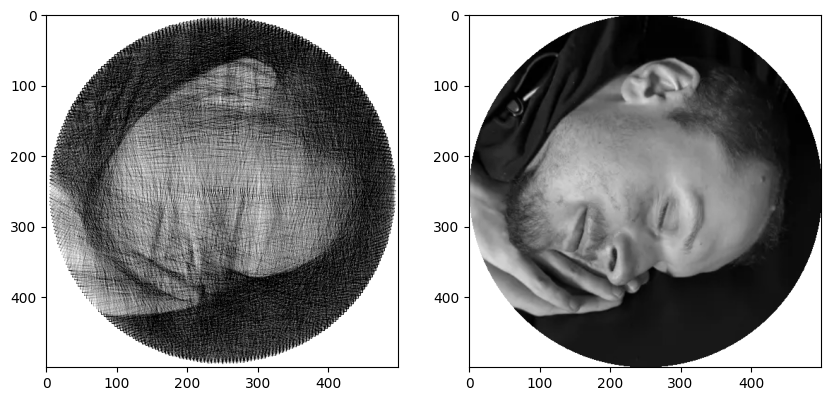
\includegraphics[width=0.8\textwidth]{dlazka.png}
	\caption{String-artová podoba spícího Dláži.}
	\label{fig:dlazka}
\end{figure}

\begin{figure}[!ht]
	\centering
	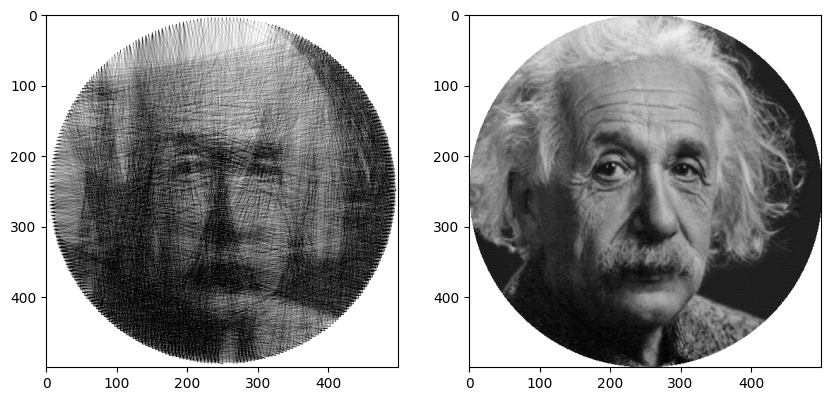
\includegraphics[width=0.8\textwidth]{einstein.png}
	\caption{String-artová podoba Einsteina.}
	\label{fig:einstein}
\end{figure}

\begin{figure}[!ht]
	\centering
	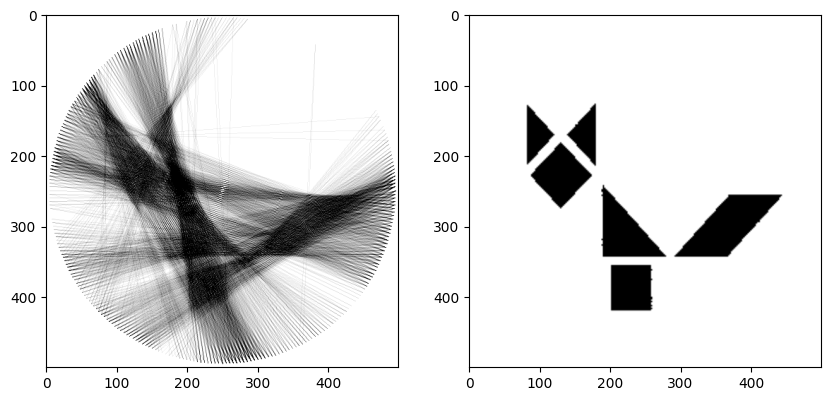
\includegraphics[width=0.8\textwidth]{logo.png}
	\caption{Logo semináře M\&M.}
	\label{fig:logo}
\end{figure}

\begin{figure}[!ht]
	\centering
	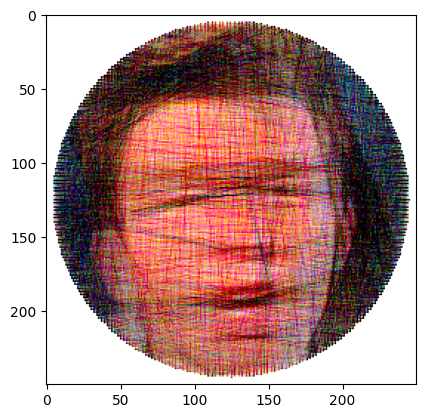
\includegraphics[width=0.4\textwidth]{rgb_rick.png}
	\caption{Barevný string-art Ricka Astleyho.}
	\label{fig:rgb_rick}
\end{figure}


\end{document}